\documentclass[]{article}
\usepackage{lmodern}
\usepackage{amssymb,amsmath}
\usepackage{ifxetex,ifluatex}
\usepackage{fixltx2e} % provides \textsubscript
\ifnum 0\ifxetex 1\fi\ifluatex 1\fi=0 % if pdftex
  \usepackage[T1]{fontenc}
  \usepackage[utf8]{inputenc}
\else % if luatex or xelatex
  \ifxetex
    \usepackage{mathspec}
  \else
    \usepackage{fontspec}
  \fi
  \defaultfontfeatures{Ligatures=TeX,Scale=MatchLowercase}
\fi
% use upquote if available, for straight quotes in verbatim environments
\IfFileExists{upquote.sty}{\usepackage{upquote}}{}
% use microtype if available
\IfFileExists{microtype.sty}{%
\usepackage{microtype}
\UseMicrotypeSet[protrusion]{basicmath} % disable protrusion for tt fonts
}{}
\usepackage[margin=1in]{geometry}
\usepackage{hyperref}
\hypersetup{unicode=true,
            pdfborder={0 0 0},
            breaklinks=true}
\urlstyle{same}  % don't use monospace font for urls
\usepackage{color}
\usepackage{fancyvrb}
\newcommand{\VerbBar}{|}
\newcommand{\VERB}{\Verb[commandchars=\\\{\}]}
\DefineVerbatimEnvironment{Highlighting}{Verbatim}{commandchars=\\\{\}}
% Add ',fontsize=\small' for more characters per line
\usepackage{framed}
\definecolor{shadecolor}{RGB}{248,248,248}
\newenvironment{Shaded}{\begin{snugshade}}{\end{snugshade}}
\newcommand{\KeywordTok}[1]{\textcolor[rgb]{0.13,0.29,0.53}{\textbf{{#1}}}}
\newcommand{\DataTypeTok}[1]{\textcolor[rgb]{0.13,0.29,0.53}{{#1}}}
\newcommand{\DecValTok}[1]{\textcolor[rgb]{0.00,0.00,0.81}{{#1}}}
\newcommand{\BaseNTok}[1]{\textcolor[rgb]{0.00,0.00,0.81}{{#1}}}
\newcommand{\FloatTok}[1]{\textcolor[rgb]{0.00,0.00,0.81}{{#1}}}
\newcommand{\ConstantTok}[1]{\textcolor[rgb]{0.00,0.00,0.00}{{#1}}}
\newcommand{\CharTok}[1]{\textcolor[rgb]{0.31,0.60,0.02}{{#1}}}
\newcommand{\SpecialCharTok}[1]{\textcolor[rgb]{0.00,0.00,0.00}{{#1}}}
\newcommand{\StringTok}[1]{\textcolor[rgb]{0.31,0.60,0.02}{{#1}}}
\newcommand{\VerbatimStringTok}[1]{\textcolor[rgb]{0.31,0.60,0.02}{{#1}}}
\newcommand{\SpecialStringTok}[1]{\textcolor[rgb]{0.31,0.60,0.02}{{#1}}}
\newcommand{\ImportTok}[1]{{#1}}
\newcommand{\CommentTok}[1]{\textcolor[rgb]{0.56,0.35,0.01}{\textit{{#1}}}}
\newcommand{\DocumentationTok}[1]{\textcolor[rgb]{0.56,0.35,0.01}{\textbf{\textit{{#1}}}}}
\newcommand{\AnnotationTok}[1]{\textcolor[rgb]{0.56,0.35,0.01}{\textbf{\textit{{#1}}}}}
\newcommand{\CommentVarTok}[1]{\textcolor[rgb]{0.56,0.35,0.01}{\textbf{\textit{{#1}}}}}
\newcommand{\OtherTok}[1]{\textcolor[rgb]{0.56,0.35,0.01}{{#1}}}
\newcommand{\FunctionTok}[1]{\textcolor[rgb]{0.00,0.00,0.00}{{#1}}}
\newcommand{\VariableTok}[1]{\textcolor[rgb]{0.00,0.00,0.00}{{#1}}}
\newcommand{\ControlFlowTok}[1]{\textcolor[rgb]{0.13,0.29,0.53}{\textbf{{#1}}}}
\newcommand{\OperatorTok}[1]{\textcolor[rgb]{0.81,0.36,0.00}{\textbf{{#1}}}}
\newcommand{\BuiltInTok}[1]{{#1}}
\newcommand{\ExtensionTok}[1]{{#1}}
\newcommand{\PreprocessorTok}[1]{\textcolor[rgb]{0.56,0.35,0.01}{\textit{{#1}}}}
\newcommand{\AttributeTok}[1]{\textcolor[rgb]{0.77,0.63,0.00}{{#1}}}
\newcommand{\RegionMarkerTok}[1]{{#1}}
\newcommand{\InformationTok}[1]{\textcolor[rgb]{0.56,0.35,0.01}{\textbf{\textit{{#1}}}}}
\newcommand{\WarningTok}[1]{\textcolor[rgb]{0.56,0.35,0.01}{\textbf{\textit{{#1}}}}}
\newcommand{\AlertTok}[1]{\textcolor[rgb]{0.94,0.16,0.16}{{#1}}}
\newcommand{\ErrorTok}[1]{\textcolor[rgb]{0.64,0.00,0.00}{\textbf{{#1}}}}
\newcommand{\NormalTok}[1]{{#1}}
\usepackage{graphicx,grffile}
\makeatletter
\def\maxwidth{\ifdim\Gin@nat@width>\linewidth\linewidth\else\Gin@nat@width\fi}
\def\maxheight{\ifdim\Gin@nat@height>\textheight\textheight\else\Gin@nat@height\fi}
\makeatother
% Scale images if necessary, so that they will not overflow the page
% margins by default, and it is still possible to overwrite the defaults
% using explicit options in \includegraphics[width, height, ...]{}
\setkeys{Gin}{width=\maxwidth,height=\maxheight,keepaspectratio}
\IfFileExists{parskip.sty}{%
\usepackage{parskip}
}{% else
\setlength{\parindent}{0pt}
\setlength{\parskip}{6pt plus 2pt minus 1pt}
}
\setlength{\emergencystretch}{3em}  % prevent overfull lines
\providecommand{\tightlist}{%
  \setlength{\itemsep}{0pt}\setlength{\parskip}{0pt}}
\setcounter{secnumdepth}{0}
% Redefines (sub)paragraphs to behave more like sections
\ifx\paragraph\undefined\else
\let\oldparagraph\paragraph
\renewcommand{\paragraph}[1]{\oldparagraph{#1}\mbox{}}
\fi
\ifx\subparagraph\undefined\else
\let\oldsubparagraph\subparagraph
\renewcommand{\subparagraph}[1]{\oldsubparagraph{#1}\mbox{}}
\fi

%%% Use protect on footnotes to avoid problems with footnotes in titles
\let\rmarkdownfootnote\footnote%
\def\footnote{\protect\rmarkdownfootnote}

%%% Change title format to be more compact
\usepackage{titling}

% Create subtitle command for use in maketitle
\newcommand{\subtitle}[1]{
  \posttitle{
    \begin{center}\large#1\end{center}
    }
}

\setlength{\droptitle}{-2em}
  \title{}
  \pretitle{\vspace{\droptitle}}
  \posttitle{}
  \author{}
  \preauthor{}\postauthor{}
  \date{}
  \predate{}\postdate{}


\begin{document}

\% The FLR platform and the a4a initiative \% FLR Team \% August 2014

\section{Why, oh why?}\label{why-oh-why}

Schnute \emph{et al.} (2007 and 1998) compared the number of software
tools and languages currently available for stock assessments with the
Babel tower myth and concluded that: ``The cosmic plan for
\textbf{confounding software languages} seems to be working remarkably
well among the community of quantitative fishery scientists!''

\section{A brief history of FLR}\label{a-brief-history-of-flr}

\begin{itemize}
\tightlist
\item
  Started by FEMS FP5, COMMIT \& EFIMAS FP6
\item
  Beta ICES WG Methods 2004
\item
  FLCore version 1.0 - 2005
\item
  FLCore version 1.4 \emph{The Golden Jackal} - 2007
  \hfill
\includegraphics[keepaspectratio, height=0.15\textheight]{graphics/WolfGoldenJackal.jpg}
\item
  FLCore version 2.2 \emph{Swordfish Polka} - 2010
  \hfill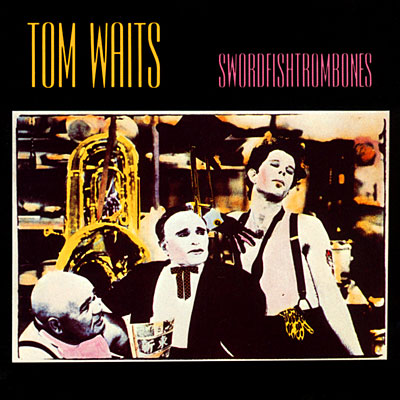
\includegraphics[keepaspectratio, height=0.15\textheight]{graphics/flr20.png}
\item
  FLR 2.4 \emph{The Duke of Prawns} - 2011
  \hfill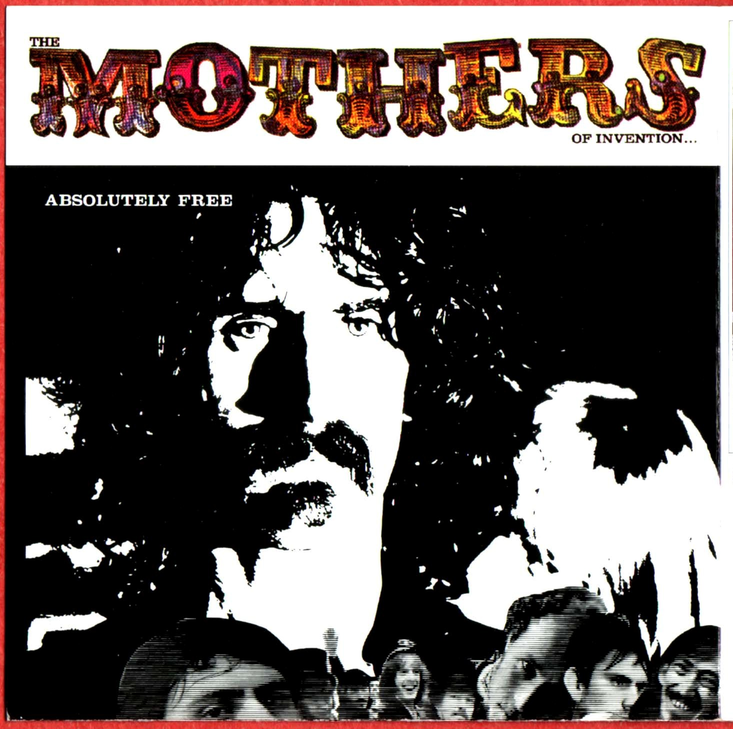
\includegraphics[keepaspectratio, height=0.15\textheight]{graphics/flr24.png}
\end{itemize}

\section{}\label{section}

\centering
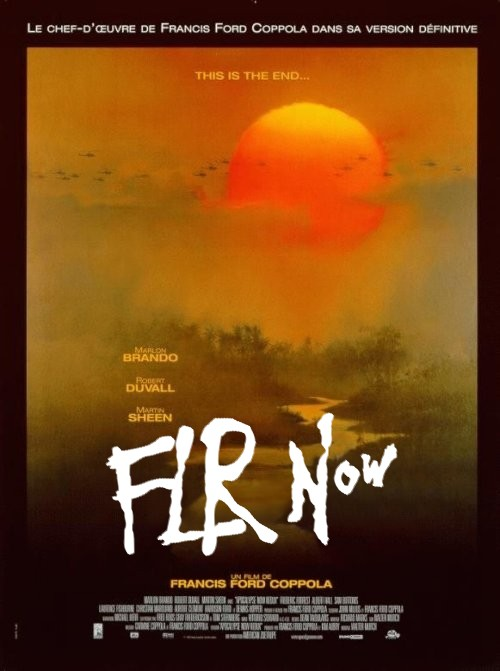
\includegraphics[keepaspectratio, height=0.85\textheight]{graphics/flr30.png}

\section{Current}\label{current}

\begin{itemize}
\tightlist
\item
  FLR 2.5.*, in continuous development
\item
  Main packages are stable
\item
  Keep track of versions you used: local copies, github or packrat
\item
  FLR 2.6 - \emph{Black Swan}
  \hfill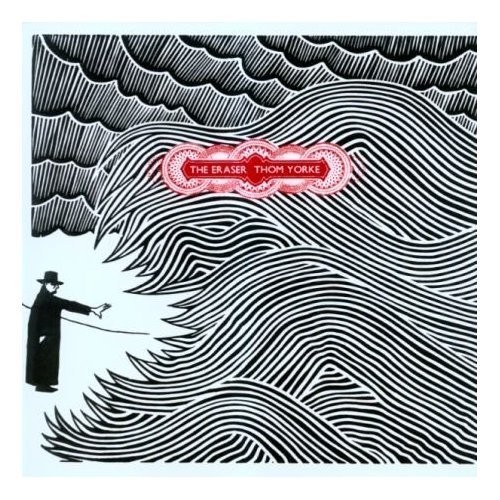
\includegraphics[keepaspectratio, height=0.15\textheight]{graphics/theeraser.jpg}
\end{itemize}

\section{FLR development}\label{flr-development}

\begin{itemize}
\tightlist
\item
  Collaborative development
\item
  Informal team
\item
  Indirect funding
\item
  Open Source
\end{itemize}

\section{\texorpdfstring{GNU project
(\url{http://gnu.org})}{GNU project (http://gnu.org)}}\label{gnu-project-httpgnu.org}

\centering

\emph{Free software is a matter of liberty, not price}

\medskip

\Huge{free = free speech}

\medskip

\Huge{free != free beer}

\section{Mission statement}\label{mission-statement}

The FLR project provides a \textbf{platform for quantitative fisheries
science} based on the R statistical language. The guiding principles of
FLR are:

\begin{itemize}
\tightlist
\item
  \textbf{openness} - through community involvement and the open source
  ethos
\item
  \textbf{flexibility} - through a design that does not constrain the
  user to a given paradigm
\item
  \textbf{extendibility} - through the provision of tools that are ready
  to be personalized and adapted.
\end{itemize}

\section{Really, what is FLR?}\label{really-what-is-flr}

\begin{itemize}
\tightlist
\item
  Extendable toolbox for implementing bio-economic simulation models of
  fishery systems
\item
  Tools used by managers (hopefully) as well as scientists
\item
  With many applications including:

  \begin{itemize}
  \tightlist
  \item
    Fit stock-recruitment relationships,
  \item
    Model fleet dynamics (including economics),
  \item
    Simulate and evaluate management procedures and HCRs,
  \item
    More than just stock assessment (VPA, XSA, ICES uptake)
  \end{itemize}
\item
  A software platform for quantitative fisheries science
\item
  A collection of R packages
\item
  A team of devoted developers
\item
  A community of active users
\end{itemize}

\section{Design principles}\label{design-principles}

\begin{itemize}
\tightlist
\item
  OOP - S4
\item
  Classes: elements in system

  \begin{itemize}
  \tightlist
  \item
    \texttt{FLStock}, fish stock

    \begin{itemize}
    \tightlist
    \item
      \texttt{FLBRP} inputs for BRP calc
    \end{itemize}
  \end{itemize}
\item
  Methods: link objects
\item
  Mid-steepenes learning curve
\end{itemize}

\section{Packages}\label{packages}

\centering
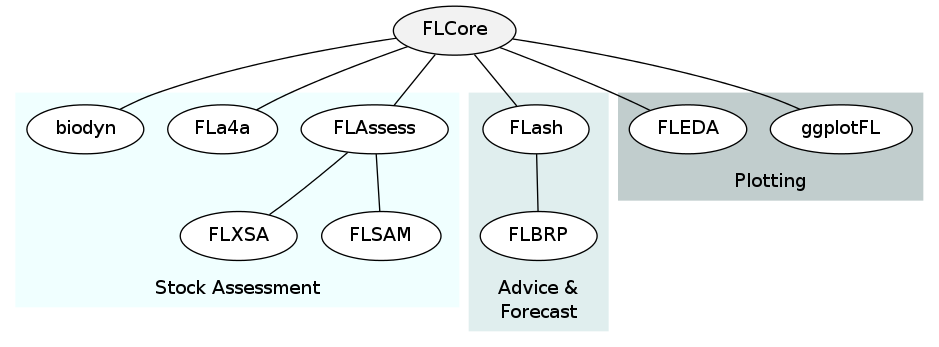
\includegraphics[keepaspectratio, width=0.95\textwidth]{graphics/flrpkgs.png}

\section{a4a - Assessment for All}\label{a4a---assessment-for-all}

\subsection{Long term vision}\label{long-term-vision}

\begin{itemize}
\tightlist
\item
  Standard methods to apply rapidly to a large number of stocks
\item
  No strong statistical technical background
\item
  Using technical knowledge on the fisheries, stocks and ecosystem
\end{itemize}

\subsection{Why}\label{why}

\begin{itemize}
\tightlist
\item
  Demand for abundance and exploitation estimates
\item
  Large investments in collecting information
\item
  Scientific advice for fisheries management.
\end{itemize}

\section{a4a - Sampled species (PT)}\label{a4a---sampled-species-pt}

\centering
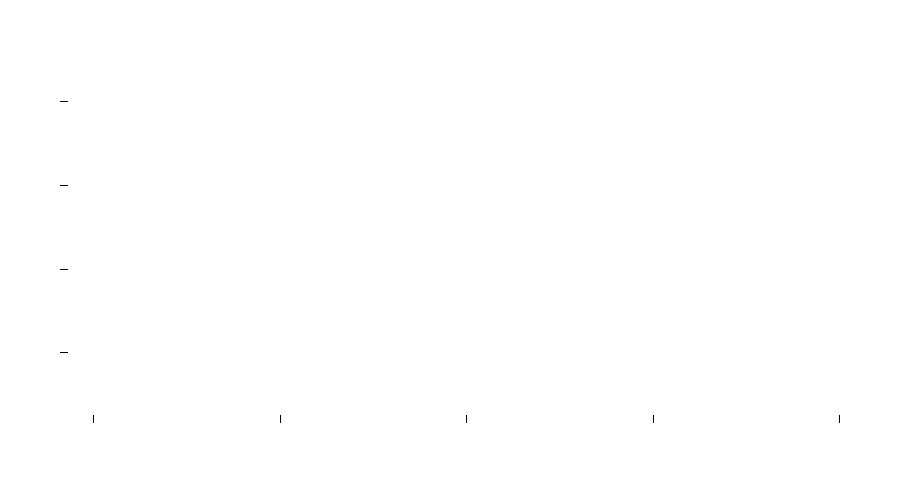
\includegraphics[keepaspectratio, height=0.6\textheight]{graphics/pt.png}

\begin{quote}
\textbf{What if we have to assess hundreds of stocks?} Estimate what you
know, simulate what you don't
\end{quote}

\section{a4a Initiative EC JRC}\label{a4a-initiative-ec-jrc}

\begin{enumerate}
\def\labelenumi{\arabic{enumi}.}
\tightlist
\item
  Develop a4a SA method
\item
  Discussion on \emph{massive} stock assessment
\item
  Capacity building (this course)
\end{enumerate}

\centering
\url{https://fishreg.jrc.ec.europa.eu/web/a4a}

\section{a4a SA model}\label{a4a-sa-model}

\begin{itemize}
\tightlist
\item
  \emph{Moderate} data stock (Catch, Survey/CPUE, little bio)
\item
  NL CaA model, R/FLR/ADMB
\item
  \emph{Simple} syntax
\end{itemize}

\begin{Shaded}
\begin{Highlighting}[]
\NormalTok{>}\StringTok{ }\NormalTok{fmodel =}\StringTok{ }\KeywordTok{separable}\NormalTok{()}
\NormalTok{>}\StringTok{ }\NormalTok{qmodel =}\StringTok{ }\KeywordTok{trawl}\NormalTok{(}\DataTypeTok{techcreep=}\FloatTok{0.03}\NormalTok{)}
\NormalTok{>}\StringTok{ }\NormalTok{rmodel =}\StringTok{ }\KeywordTok{beverton}\NormalTok{(}\DataTypeTok{a=}\KeywordTok{s}\NormalTok{(NAO))}
\end{Highlighting}
\end{Shaded}

\section{a4a MSE}\label{a4a-mse}

Building an STANDARD MSE

\begin{enumerate}
\def\labelenumi{\arabic{enumi}.}
\tightlist
\item
  OM uncertainty in growth, S/R and selectivity
\item
  HCRs based on catch, surveys, assessments
\item
  Assessment models of increasing complexity
\item
  OE for catch and index
\item
  IE in F or catch
\end{enumerate}

\section{MSE - The Lego block
approach}\label{mse---the-lego-block-approach}

\centering
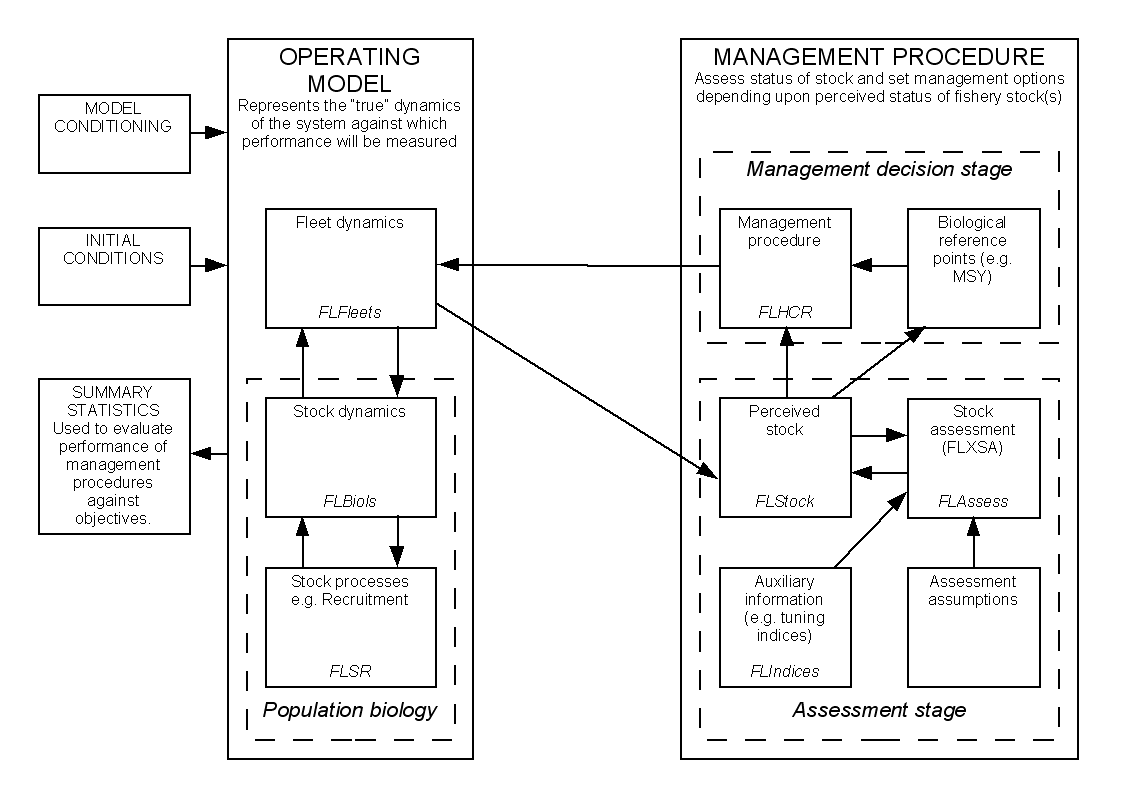
\includegraphics[keepaspectratio, height=0.8\textheight]{graphics/MSE.png}

\section{More information}\label{more-information}

\begin{itemize}
\tightlist
\item
  \href{http://flr-project.org}{FLR Project @ http://flr-project.org}
\item
  \href{http://gtihub.com/flr/}{Source code @ http://github.com/flr/}
\item
  \href{https://fishreg.jrc.ec.europa.eu/web/a4a}{a4a Initiative @
  https://fishreg.jrc.ec.europa.eu/web/a4a}
\end{itemize}

\section{}\label{section-1}

\centering

\includegraphics[keepaspectratio, height=0.8\textheight]{graphics/keep-calm-and-code-flr.png}


\end{document}
